\documentclass[12pt]{article}

\setlength{\parindent}{0pt}
\setcounter{secnumdepth}{3}
\usepackage[margin=1in]{geometry}

% packages
\usepackage{amsmath, amsfonts, amsthm, amssymb}
\usepackage{graphicx, float}
\usepackage{mathtools}
\usepackage{titlesec}
\usepackage{interval}
\usepackage{hyperref}
\usepackage{siunitx}
\usepackage{titling}
\usepackage{vwcol}
\usepackage{setspace}
\usepackage{empheq}
\usepackage{cancel}
\usepackage{esdiff}
\usepackage{multicol}
\usepackage{mdframed}
\usepackage{esdiff}
\usepackage{tikzsymbols}
\usepackage{multicol}
\usepackage{tikz}
\usepackage{varwidth}
\usepackage{pgfplots}
\usepackage{fancyhdr}
\usepackage{enumitem}
\usepackage{tcolorbox}

\intervalconfig {
	soft open fences
}

% header
\pagestyle{fancy}
\fancyhf{}
\lhead{Ethan Fan}
\rhead{PCH}
\cfoot{\thepage}

% section format
\titleformat{\section}
  {\bfseries}
  {}
  {0em}
  {}
\titlespacing*{\section}{0pt}{0pt}{0.3em}

\titleformat{\subsection}[runin]
  {\bfseries}
  {}
  {0em}
  {}
\titlespacing*{\subsection}{0pt}{0pt}{0em}

\titleformat{\subsubsection}[runin]
  {\itshape}
  {(\roman{subsubsection})}
  {0em}
  {}

% commands
\newcommand{\alignedintertext}[1]{%
  \noalign{%
    \vskip\belowdisplayshortskip
    \vtop{\hsize=\linewidth#1\par
    \expandafter}%
    \expandafter\prevdepth\the\prevdepth
  }%
}

\newcommand*{\paren}[1]{\ensuremath\left(#1\right)}
\newcommand*{\limit}[2][x]{\ensuremath{\displaystyle\lim_{#1\to#2}}}
\newcommand*{\Limit}[3][x]{\ensuremath{\displaystyle\lim_{#1\to#2}\left[#3\right]}}
\newcommand*{\deriv}[1][x]{\ensuremath{\dfrac{\mathrm{d}}{\mathrm{d}#1}}}
\newcommand*{\Deriv}[2][x]{\ensuremath{\dfrac{\mathrm{d}}{\mathrm{d}#1}\left[#2\right]}}
\newcommand{\dydx}{\frac{dy}{dx}}
\newcommand*{\iinteg}[2][x]{\ensuremath{\displaystyle\int #2\;\mathrm{d}#1}}
\newcommand*{\dinteg}[4][x]{\ensuremath{\displaystyle\int_{#2}^{#3}#4\;\mathrm{d}#1}}
\newcommand*{\abs}[1]{\ensuremath{\left|#1\right|}}
\newcommand*{\eps}{\varepsilon}
\newcommand*{\cbrt}[1]{\ensuremath{\sqrt[3]{#1}}}
\newcommand*{\lheqzero}{\ensuremath{\underset{\text{L'H}}{\overset{\left[\frac00\right]}{=}}}}
\newcommand*{\lheqinfty}{\ensuremath{\underset{\text{L'H}}{\overset{\left[\frac{\infty}{\infty}\right]}{=}}}}
\newcommand{\tor}{\text{ or }}
\newcommand{\floor}[1]{\lfloor #1 \rfloor}

\newcommand{\vem}{\vspace{0.5em}}
\newcommand{\example}[1]{\section{Example #1}}
\newcommand{\problem}[1]{\section{Problem #1}}
\newcommand{\subproblem}[1]{\subsection{(#1)} \,}

\DeclareMathOperator{\dne}{DNE}
\DeclareMathOperator{\sgn}{sgn}

\newcommand{\definition}[1]{\begin{tcolorbox}[colback=red!5!white,colframe=red!75!black,parbox=false] #1 \end{tcolorbox}}

\newcommand{\theorem}[2]{\begin{tcolorbox}[title={#1},colback=blue!5!white,colframe=blue!75!black,parbox=false] #2 \end{tcolorbox}}

\allowdisplaybreaks
% \postdisplaypenalty=100000

% document
\begin{document}

\vspace*{0cm}

% opening
\begin{center}
    {\Large \bfseries Problem Set 62} \\[0.5cm]
    {\large Derivatives 1} \\[0.35cm]
    {\normalsize April 7, 2026}
\end{center}

% problems

\problem{1}
Find $f'(a)$ using the limit process:
\subproblem{a} $f(x)=\dfrac{2x+1}{x+3}$
\begin{align*}
f(x)=&\dfrac{2x+1}{x+3}=\frac{-5}{x+3}+2\\
  f'(x)=&\lim_{h \to 0} \frac{f(x+h)-f(x)}{h}\\=&\lim_{h \to 0}\frac{\frac{-5}{x+h+3}+2-\frac{-5}{x+3}-2}{h}\\=&\lim_{h \to 0}\frac{\frac{5}{x+3}-\frac{5}{x+h+3}}{h}\\=&\lim_{h \to 0}\frac{\frac{5h}{(x+3)(x+h+3)}}{h}\\=&\lim_{h \to 0}\frac{5}{(x+3)(x+h+3)}\\
  =&\boxed{\frac{5}{x^3+6x+9}}
\end{align*}

\problem{4}
Let $f(x)=\dfrac{(2^x+2^{-x})\sin x\sqrt{\arctan (x^2-x+1)}}{(7x^2+3x+1)^3}$. Use the limit definition of the derivative to find the value of $f'(0)$.
\begin{align*}
    f'(0)
    =&\limit{0} \frac{f(x)-f(0)}{x-0}\\
    =&\limit{0} \frac{\frac{(2^x+2^{-x})\sin x\sqrt{\arctan (x^2-x+1)}}{(7x^2+3x+1)^3}-\frac{(2^0+2^{-0})\sin 0\sqrt{\arctan (0^2-0+1)}}{(7\cdot0^2+3\cdot0+1)^3}}{x}\\
    =&\limit{0} \frac{\frac{(2^x+2^{-x})\sin x\sqrt{\arctan (x^2-x+1)}}{(7x^2+3x+1)^3}}{x}\\
    =&\limit{0} \frac{(2^x+2^{-x})\sqrt{\arctan (x^2-x+1)}}{(7x^2+3x+1)^3} \cdot \frac{\sin x}{x}\\
    =&\limit{0} \frac{(1+1)\sqrt{\arctan1}}{1^3}\\
    =& 2\sqrt{\frac{\pi}{4}} = \boxed{\sqrt{\pi}}
\end{align*}

\theorem{Theorem 1 Differentiability implies Continuity}{If $f$ is differentiable at $a$, then $f$ is continuous at $a$.\vspace{0.5em}\\ 
Note: The converse of Theorem 1 is false; that is, there are functions that are continuous but not differentiable.}

\problem{5}
Prove Theorem 1. \vspace{0.5em} \\
Given that $f(x)$ is differentiable at $a$,
\begin{align*}
    \limit{a}f(x)-f(a)=& \limit{a}(f(x)-f(a))\\
    =& \limit{a}(\frac{(f(x)-f(a))(x-a)}{x-a})\\
    =& \limit{a}(\frac{f(x)-f(a)}{x-a})\limit{a}(x-a)\\
    =& f'(a) \cdot 0\\
    =&0 
\end{align*}\vspace{-1.5em}
\[
\boxed{\limit{a}f(x)=f(a)}
\]
Therefore, $f(x)$ is continuous on $a$. \vem

\problem{7}
Discuss the differentiability of
\subproblem{b} $f(x)=\begin{cases}
    \dfrac{\sin x^2}{x} &\text{if $x\ne 0$} \\
    0  &\text{if $x=0$}
\end{cases}$ at $x=0$
\begin{gather*}
    f_-'(0)=\lim_{h \to 0^-} \frac{\frac{\sin h^2}{h}-0}{h}=\lim_{h \to 0^-} \frac{\sin h^2}{h^2}=1\\
    f_+'(0)=\lim_{h \to 0^+} \frac{\frac{\sin h^2}{h}-0}{h}=\lim_{h \to 0^+} \frac{\sin h^2}{h^2}=1\\
    f_-'(0)=f_+'(0)=1 \implies f'(0)=1\\
    \boxed{\text{$f(x)$ is differentiable at $x=0$}}
\end{gather*}

\subproblem{c} $f(x)=\begin{cases}
    x \sin (\ln x^2) &\text{if $x\ne 0$} \\
    0  &\text{if $x=0$}
\end{cases}$ at $x=0$
\begin{gather*}
    f_-'(0)=\lim_{h \to 0^-} \frac{h \sin (\ln h^2)-0}{h}=\lim_{h \to 0^-} \sin (\ln h^2) \dne \\
    f_+'(0)=\lim_{h \to 0^+} \frac{h \sin (\ln h^2)-0}{h}=\lim_{h \to 0^+} \sin (\ln h^2) \dne \\
    f_-'(0) \dne, f_+'(0) \dne \implies f'(0) \dne \\
    \boxed{\text{$f(x)$ is not differentiable at $x=0$}}
\end{gather*}

\problem{8}
Trace or copy the graph of the given function $f$. (Assume that the axes have equal scales.) Then sketch
the graph of $f'$ below it.
\begin{figure}[H]
    \centering
    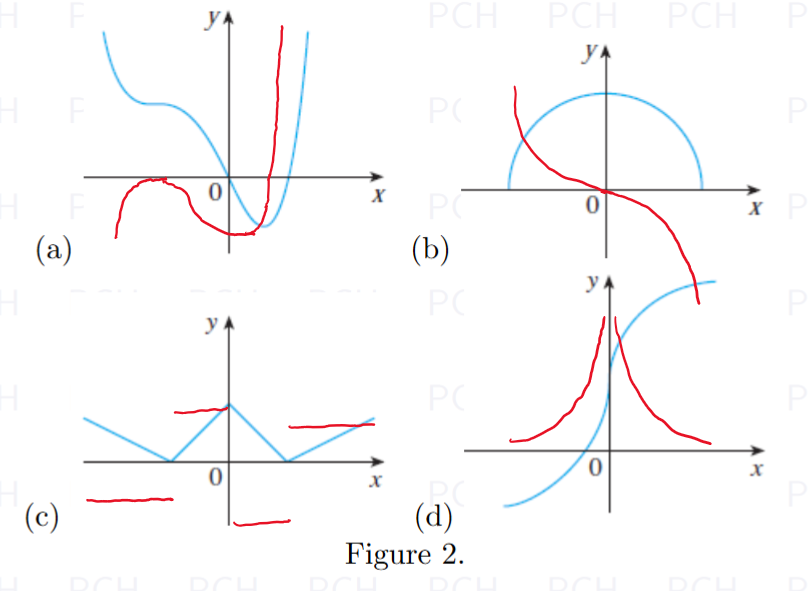
\includegraphics[width=0.6\linewidth]{figure2.png}
    \label{fig:placeholder}
\end{figure}

\problem{9}
The figure shows the graphs of $f$, $f'$, and $f''$. Identify each curve, and explain your choices.
\begin{figure}[H]
    \centering
    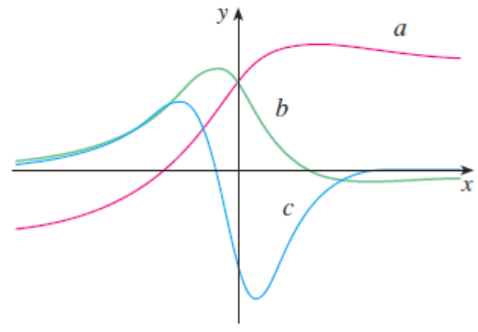
\includegraphics[width=0.5\linewidth]{figure3.png}
    \label{fig:placeholder}
\end{figure}
\begin{gather*}
    a'=0, b=0 \implies a'=b\\
    b'=0, c=0 \implies b'=c\\
    \boxed{f=a,f'=b,f''=c}
\end{gather*}

\problem{10}
The figure shows the graphs of three functions. One is the position function of a car, and one is the velocity
of the car, and one is its acceleration. Identify each curve, and explain your choices.
\begin{figure}[H]
    \centering
    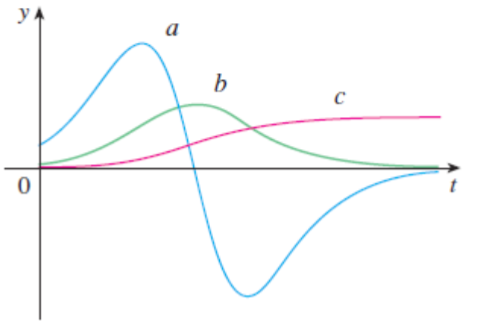
\includegraphics[width=0.4\linewidth]{figure4.png}
\end{figure}
\begin{gather*}
    c'=0, b=0 \implies c'=b\\
    b'=0, a=0 \implies b'=a\\
    \boxed{f=c,f'=b,f''=a}
\end{gather*}

\problem{11}
Use the limit definition of a derivative to find $f'$ and $f''$. Then graph $f$, $f'$, and $f''$ on a common screen and check to see if your answers are reasonable.
\begin{equation*}
   f(x)=1+4x-x^2 
\end{equation*}
\begin{align*}
    f'(x)=&\limit{h} \frac{f(x+h)-f(x)}{h}\\
    =&\limit{h} \frac{1+4(x+h)-(x+h)^2-1-4x+x^2}{h}\\
    =&\limit{h} \frac{4h-2hx-h^2}{h}\\
    =&\limit{h}4-2x-h\\
    =&\boxed{4-2x}\\
    f''(x)=&\limit{h} \frac{f'(x+h)-f'(x)}{h}\\
    =&\limit{h} \frac{4-2x-2h-4+2x}{h}\\
    =&\limit{h} \frac{2h}{h}\\
    =&\boxed{2}
\end{align*}

\begin{figure}[H]
    \centering
    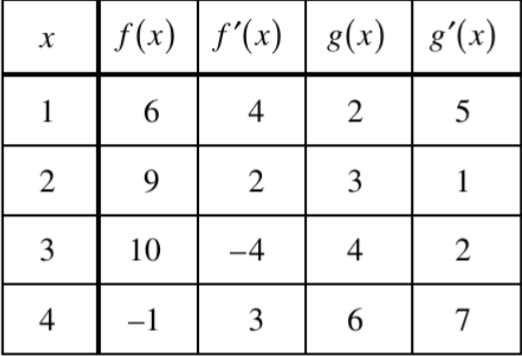
\includegraphics[width=0.4\linewidth]{figure5.png}
    \label{fig:placeholder}
\end{figure}
\problem{13}
The functions $f$ and $g$ are differentiable for all real numbers, and $g$ is strictly increasing. The table above gives values of the functions and their derivatives at selected values of $x$. The function $h$ is given by $h(x) = f (g(x)) - 6$. Explain why there must be a value $r$ for $1 < r < 3$ such that $h(r) = -5$.
\begin{gather*}
    h(r)=f(g(r))-6=-5 \implies f(g(r))=1\\
    f(3)=10, f(4)=-1 \implies 10<f(g(r))<-1\\
    3<g(r)<4 \implies 2<r<3
\end{gather*}
By the Intermediate Theorem, since $g(x)$ is continuous on $\mathbb{R}$, and $3=g(2)<g(3)=4$, then there exist a number $r\in (2,3)$ such that $g(r)\in (3,4).$ By the Intermediate Theorem, since $f(x)$ is continuous on $\mathbb{R}$, and $-1=f(4)<f(3)=10$, the  there exist a number $g(r) \in (3,4)$ such that $f(g(r))\in (-1,10)$. Thus, $h(r)$ is able to achieve the value of $-5$.

\problem{14}
A student starts reading a book at time $t = 0$ minutes and continues reading for the next $10$ minutes.
The rate at which the student reads is modeled by the differentiable function $R$, where $R(t)$ is measured
in words per minute. Selected values of $R(t)$ (minutes) are given in the table shown.
\begin{figure}[H]
    \centering
    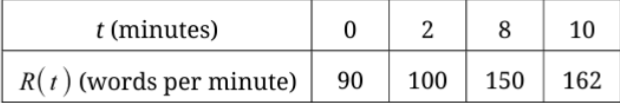
\includegraphics[width=0.5\linewidth]{figure6.png}
    \label{fig:placeholder}
\end{figure}

\subproblem{a}
Approximate $R'(1)$ using the average rate of change of $R$ over the interval $0 \le t \le 2$. Show the work
that leads to your answer. Indicate units of measure.
\[
R'(1)=\frac{100-90}{2}=\boxed{5 \text{ words/min$^2$}}
\]

\subproblem{b}
Must there be a value $c$, for $0 < c < 10$, such that $R(c) = 155$? Justify your answer. \vem \\
1. $R(t)$ is a differentiable and continuous function on [0,10].\\
2. $R(0)=90,R(10)=162$
\[
90<N<162 \implies \text{let }N=155
\]
3. By the Intermediate Value Theorem, since $R(x)$ is continuous on $[0,10]$, and $R(0)<155<R(10)$, then there exist a number $c\in (0,10)$ such that $R(c)=155$.

\end{document}

